%% ===============================================================================================
%% @author Leonardo Florez-Valencia (florez-l@javeriana.edu.co)
%% ===============================================================================================

\documentclass[letter]{article}

\usepackage[spanish]{babel}
\usepackage[margin=1in]{geometry}
\usepackage{amsmath}
\usepackage{amsthm}
\usepackage{amssymb}
\usepackage[utf8]{inputenc}
\usepackage{graphicx, color}
\usepackage{algorithm}
\usepackage{algpseudocode}
\usepackage{mathrsfs}
\graphicspath{ {graphics/} }
% Some definitions
\floatname{algorithm}{Algoritmo}

% Author info
\title{Escritura del problema de la inversión de la cadena}
\author{David Enrique Palacios García$^1$ \and Karen Sofia Coral Godoy$^1$}
\date{
	$^1$Departamento de Ingeniería de Sistemas, Pontificia Universidad Javeriana\\Bogotá,  Colombia \\
	\texttt{\{david\_palacios, corallg\_ksofia\}@javeriana.edu.co}\\~\\
	\today
}

\begin{document}
\maketitle
	
\begin{abstract}
En este documento se presenta la formalización del problema de la inversión de una cadena, junto con la descripción de dos algoritmos que lo solucionan. Además, se presenta un análisis experimental de la complejidad de esos dos algoritmos.
\textbf{Palabras clave:} inversión, algoritmo, formalización, experimentación, complejidad, cadena.
\end{abstract}

\tableofcontents
	
\section{Introducción} \label{intro}
Invertir una cadena puede llegar a ser útil para encontrar similitudes entre datos, tal así, que existe un gran número de formas para hacerlo. El ejemplo práctico que se tratará en este documento será tomar un número natural N, convertirlo a cadena binaria, invertir esta cadena y, finalmente, obtener el valor entero de la cadena invertida. Para resolver este problema se presentan dos algoritmos que lo solucionan, con el objetivo de mostrar: la formalización del problema (sección \ref{formalizacion}), la escritura formal de dos algoritmos (sección \ref{algoritmos}) y un análisis experimental de la complejidad de cada uno de ellos (sección \ref{experimentos}).

\section{Formalización del problema} \label{formalizacion}
Cuando se piensa en {\it invertir una cadena} la solución inmediata puede ser muy simplista: inocentemente, se piensa en leer una cadena de atrás hacia adelante. Sin embargo, con un poco más de reflexión, hay tres preguntas que pueden surgir:
\begin{enumerate}
  \item ¿Cadena es únicamente de tipo \texttt{String}?
  \item ¿Cómo se guardan esas cadenas en memoria?
  \item ¿Solo se pueden ordenar letras?
\end{enumerate}

Recordemos que, en memoria, una cadena de tipo \texttt{String} es un arreglo de datos de tipo caracter. Además, es necesario entender que cualquier caracter utilizado por una máquina en realidad tiene un valor \texttt{ASCII}. Esto significa que cualquier letra, símbolo o número representado por una máquina, se puede escribir como una secuencia de caracteres.
Basado en esta premisa, entendemos que convirtiendo cualquier dato en un arreglo de caracteres, podemos invertir su secuencia y obtener un nuevo dato.

\subsection{Definición del problema de la ``inversión de la cadena''} \label{problema}
Así, el problema del ordenamiento se define a partir de:
  \begin{enumerate}
    \item una secuencia $S$ de elementos $a\in \mathbb{C}$
  \end{enumerate}
producir una nueva secuencia $S'$ cuyos elementos cumplan con la relación $a_n,~ a_{n-1},~ ...~ a_0$.
\begin{itemize}
    \item Entradas:
    \begin{itemize}
        \item $S = \left< a_i \in \mathbb{C} \right> ~ | ~ 1\le i \le n$.
    \end{itemize}
    \item Salidas:
    \begin{itemize}
        \item $S' = \left< e_i \in S m\right> ~ | ~ e_n,~ e_{n-1} \forall i \in \left[1,n\right)$.
    \end{itemize}
\end{itemize}

\section{Algoritmos de solución} \label{algoritmos}
\subsection{Dividir y vencer} \label{algoritmos:dyv}
La idea de este algoritmo es: en primera medida, entender que la inversión de una cadena con un único elemento, es igual a la cadena inicial, este siendo el caso base. Por otra parte,
eligiendo un pivote en el medio de la secuencia, permite dividirla en subsecuencias de carácteres, que a su vez, son invertidas de derecha a izquierda.

\newpage

\begin{algorithm}[!htb]
\caption{Inversión de Cadena DyV: Convertir un entero a cadena de caracteres binarios.}
\begin{algorithmic}[1]
\Require $n \in \mathbb{N} $
\Ensure $S$  $= \left< e_i \in S  ~ | ~ e_i < e_{i+1} \forall i \in \left[1,n\right)\right>$
\Procedure{NaiveBubbleSort}{$S$}
  \For{$i \leftarrow 1~\mathbf{to}~|S|$}
    \For{$j \leftarrow 1~\mathbf{to}~|S|-1$}
      \If{$s_{j+1}<s_j$}
        \State \Call{Swap}{$s_j,s_{j+1}$}
      \EndIf
    \EndFor
  \EndFor
\EndProcedure
\end{algorithmic}
\end{algorithm}

\subsubsection{Análisis de complejidad} \label{algoritmos:inocente:complejidad}

Por inspección de código: hay dos ciclos {\it para-todo} anidados que, en el peor de los casos, recorren todo la secuencia de datos; entonces, este algoritmo es $O(|S|^2)$.

\subsubsection{Invariante} \label{algoritmos:inocente:invariante}

Después de cada iteración controlada por el contador $i$, los $i$ elementos más grandes quedan al final de la secuencia.

\begin{enumerate}
    \item Inicio: $i=0$, la secuencia vacía está ordenada.
    \item Iteración: $1 \le i<|S|$, si se supone que los $i-1$ elementos más grandes ya están en su posición, entonces la nueva iteración llevará los $i$-ésimo elemento a su posición adecuada.
    \item Terminación: $i=|S|$, los $|S|$ elementos más grandes están en su posición, entonces la secuencia está ordenada.
\end{enumerate}

\section{Análisis experimental} \label{experimentos}

En esta sección se presentarán algunos los experimentos para confirmar los órdenes de complejidad de los tres algoritmos presentados en la sección \ref{algoritmos}.

\subsection{Secuencias aleatorias} \label{experimentos:aleatorias}

Acá se presentan los experimentos cuando los algoritmos se ejecutan con secuencias de entrada de orden aleatorio.

\subsubsection{Protocolo}
\begin{enumerate}
    \item Cargar en memoria un archivo de, al menos, 200Kb.
    \item Definir un rango $(b,e,s)\in\mathbb{N}^3$, donde: $b$ es un tamaño inicial, $e$ es un tamaño final y $s$ es un salto. Se generarán secuencias, a partir del archivo de entrada, de diferentes tamaños desde $b$ hasta $e$, adicionando cada vez $s$ elementos.
    \item Cada algoritmo se ejecutará 5 veces con cada secuencia y se guardará el tiempo promedio de ejecución.
    \item Se generan los gráficos necesarios para comparar los algoritmos.
\end{enumerate}

\subsubsection{Experimentación}
\begin{enumerate}
    \item Se utilizó el programa \texttt{$run\_random\_experiment.py$} con los parámetros de entrada:
    \begin{itemize}
        \item \texttt{paisajeMedio.webp} con un peso de \texttt{345KB} como archivo de entrada
        \item \texttt{b=0} como tamaño inicial del arreglo
        \item \texttt{e=10000} como tamaño final del arreglo
        \item \texttt{s=100} como saltos entre iteraciones del algoritmo
    \end{itemize}
    \item El programa logró finalizar sin complicaciones, con un tiempo estimado de 2 horas.
    \item Se obtuvieron 100 datos con el tiempo promedio de cada uno de los algoritmos, logrando así crear la siguiente gráfica: (ver Figura 1)
\end{enumerate}

\begin{figure}[h]
    \centering
    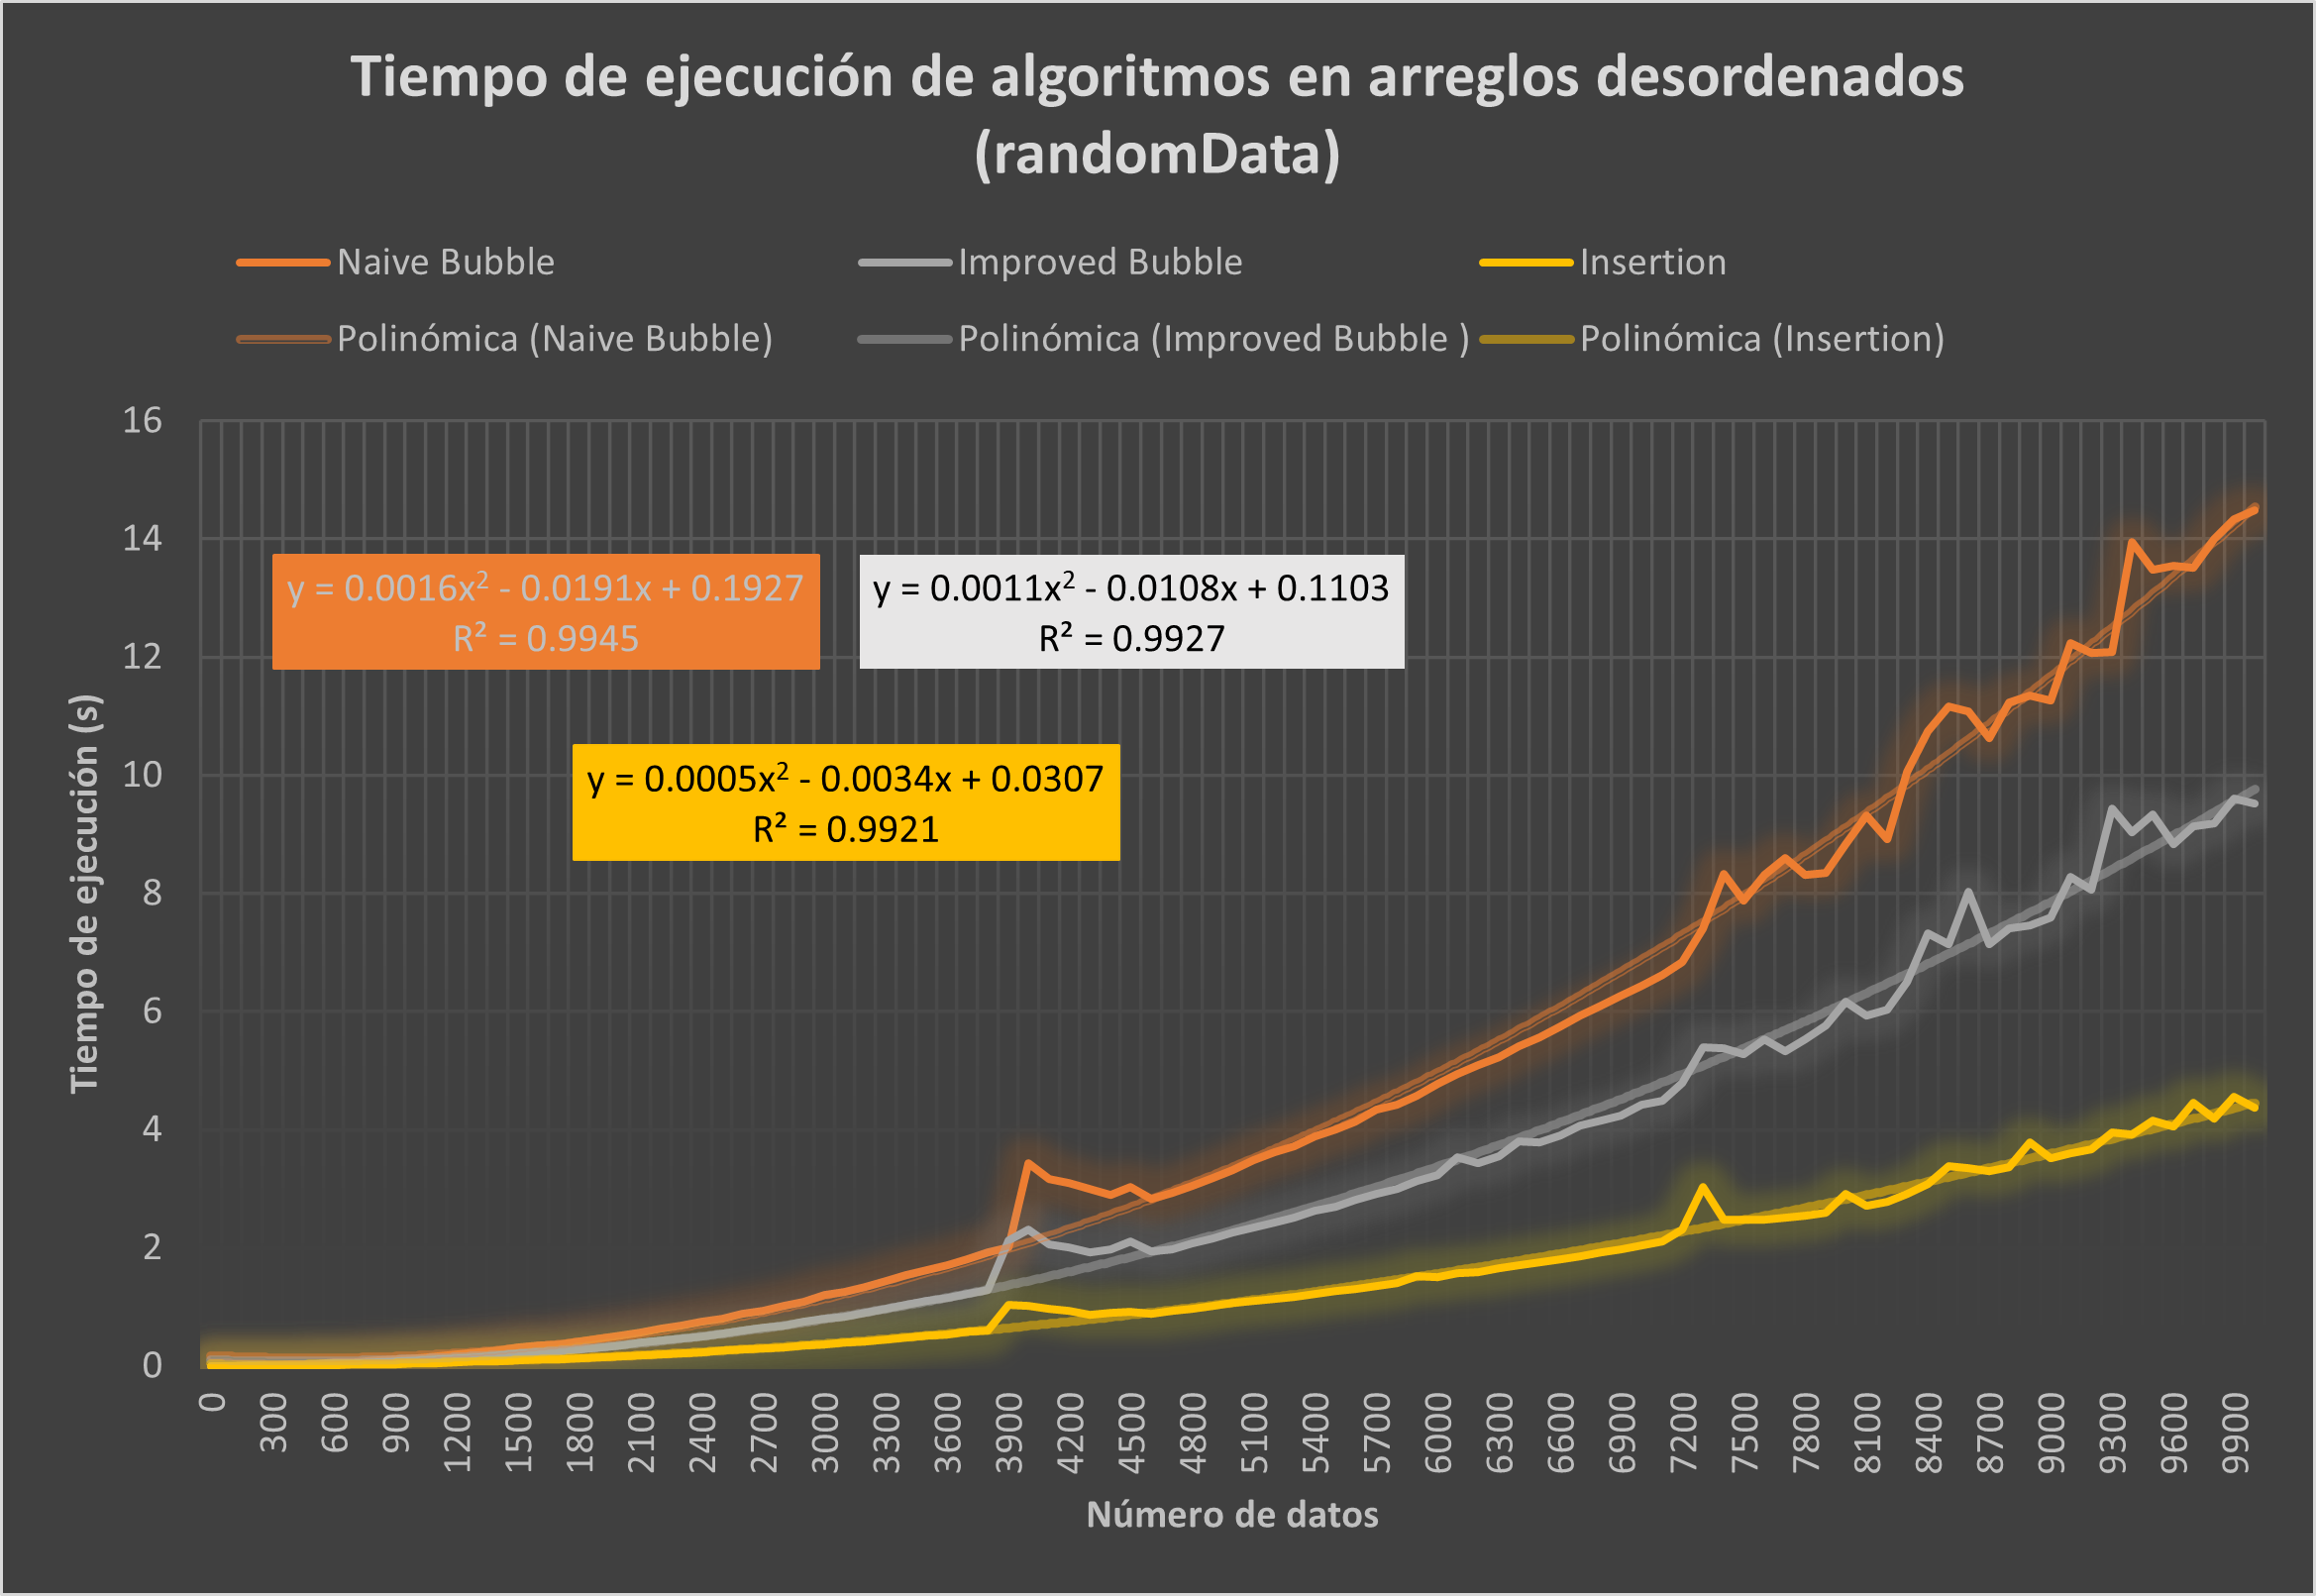
\includegraphics[scale=0.76]{randomDataGraphic.png}
    \label{experimentos:aleatorias:grafica}
    \caption{Tiempo de ejecución de los algoritmos con datos desordenados}
\end{figure}

\subsubsection{Análisis del experimento}
\label{experimentos:aleatorias:analisis}
Como se puede notar, en este caso los 3 algoritmos tienen una complejidad $\Theta(n^{2})$, sin embargo, a partir de arreglos de 1500 datos, se empiezan a notar diferencias entre ellos. La principal es que es evidente que, aunque no deja de ser cuadrática, el $Insertion Sort$ es mucho más rápido que el $Bubble Sort Inocente$ y su contraparte mejorada. Eso sí, también se evidencia la mejoría del $Bubble Sort$ aplicando la correción estudiada anteriormente.

Así mismo, utilizando herramientas de Microsoft Excel, se pudo aplicar una regresión cuadrática, hallando las lineas de tendencia de cada algoritmo, su ecuación y valor $R^{2}$ que estaban muy cercanos a 1, lo cual indica que se aplico el modelo más preciso, y por ende se reafirma la complejidad algorítmica $O(|S|^2)$ de las soluciones presentadas.

\subsection{Secuencias ordenadas} \label{experimentos:ordenadas}

Acá se presentan los experimentos cuando los algoritmos se ejecutan con secuencias de entrada ordenadas de acuerdo al orden parcial $a<b$.

\subsubsection{Protocolo}
\begin{enumerate}
    \item Definir un rango $(b,e,s)\in\mathbb{N}^3$, donde: $b$ es un tamaño inicial, $e$ es un tamaño final y $s$ es un salto. Se generarán secuencias aleatorias de diferentes tamaños desde $b$ hasta $e$, adicionando cada vez $s$ elementos.
    \item Se usará el algoritmo \texttt{sort(S)}, disponible en la librería básica de python, para ordenar dicha secuencia.
    \item Cada algoritmo se ejecutará 5 veces con cada secuencia ordenada y se guardará el tiempo promedio de ejecución.
    \item Se generan los gráficos necesarios para comparar los algoritmos.
\end{enumerate}

\subsubsection{Experimentación}
\begin{enumerate}
    \item Se utilizó el programa \texttt{$run\_sorted\_experiment.py$} con los parámetros de entrada:
    \begin{itemize}
        \item \texttt{b=0} como tamaño inicial del arreglo
        \item \texttt{e=10000} como tamaño final del arreglo
        \item \texttt{s=100} como saltos entre iteraciones del algoritmo
    \end{itemize}
    \item Se creó un arreglo de tamaño \texttt{e} con números aleatorios entre -1000000 y 1000000.
    \item Utilizando la función \texttt{sort(S)} de la librería básica de Pyhton, se ordena ascendentemente el arreglo y se empiezan a ejecutar los algoritmos. 
    \item El programa logró finalizar sin complicaciones, con un tiempo estimado de hora y media.
    \item Se obtuvieron 100 datos con el tiempo promedio de cada uno de los algoritmos, logrando así crear la siguiente gráfica: (ver Figura 2)
\end{enumerate}
\newpage


\begin{figure}[h]
    \centering
    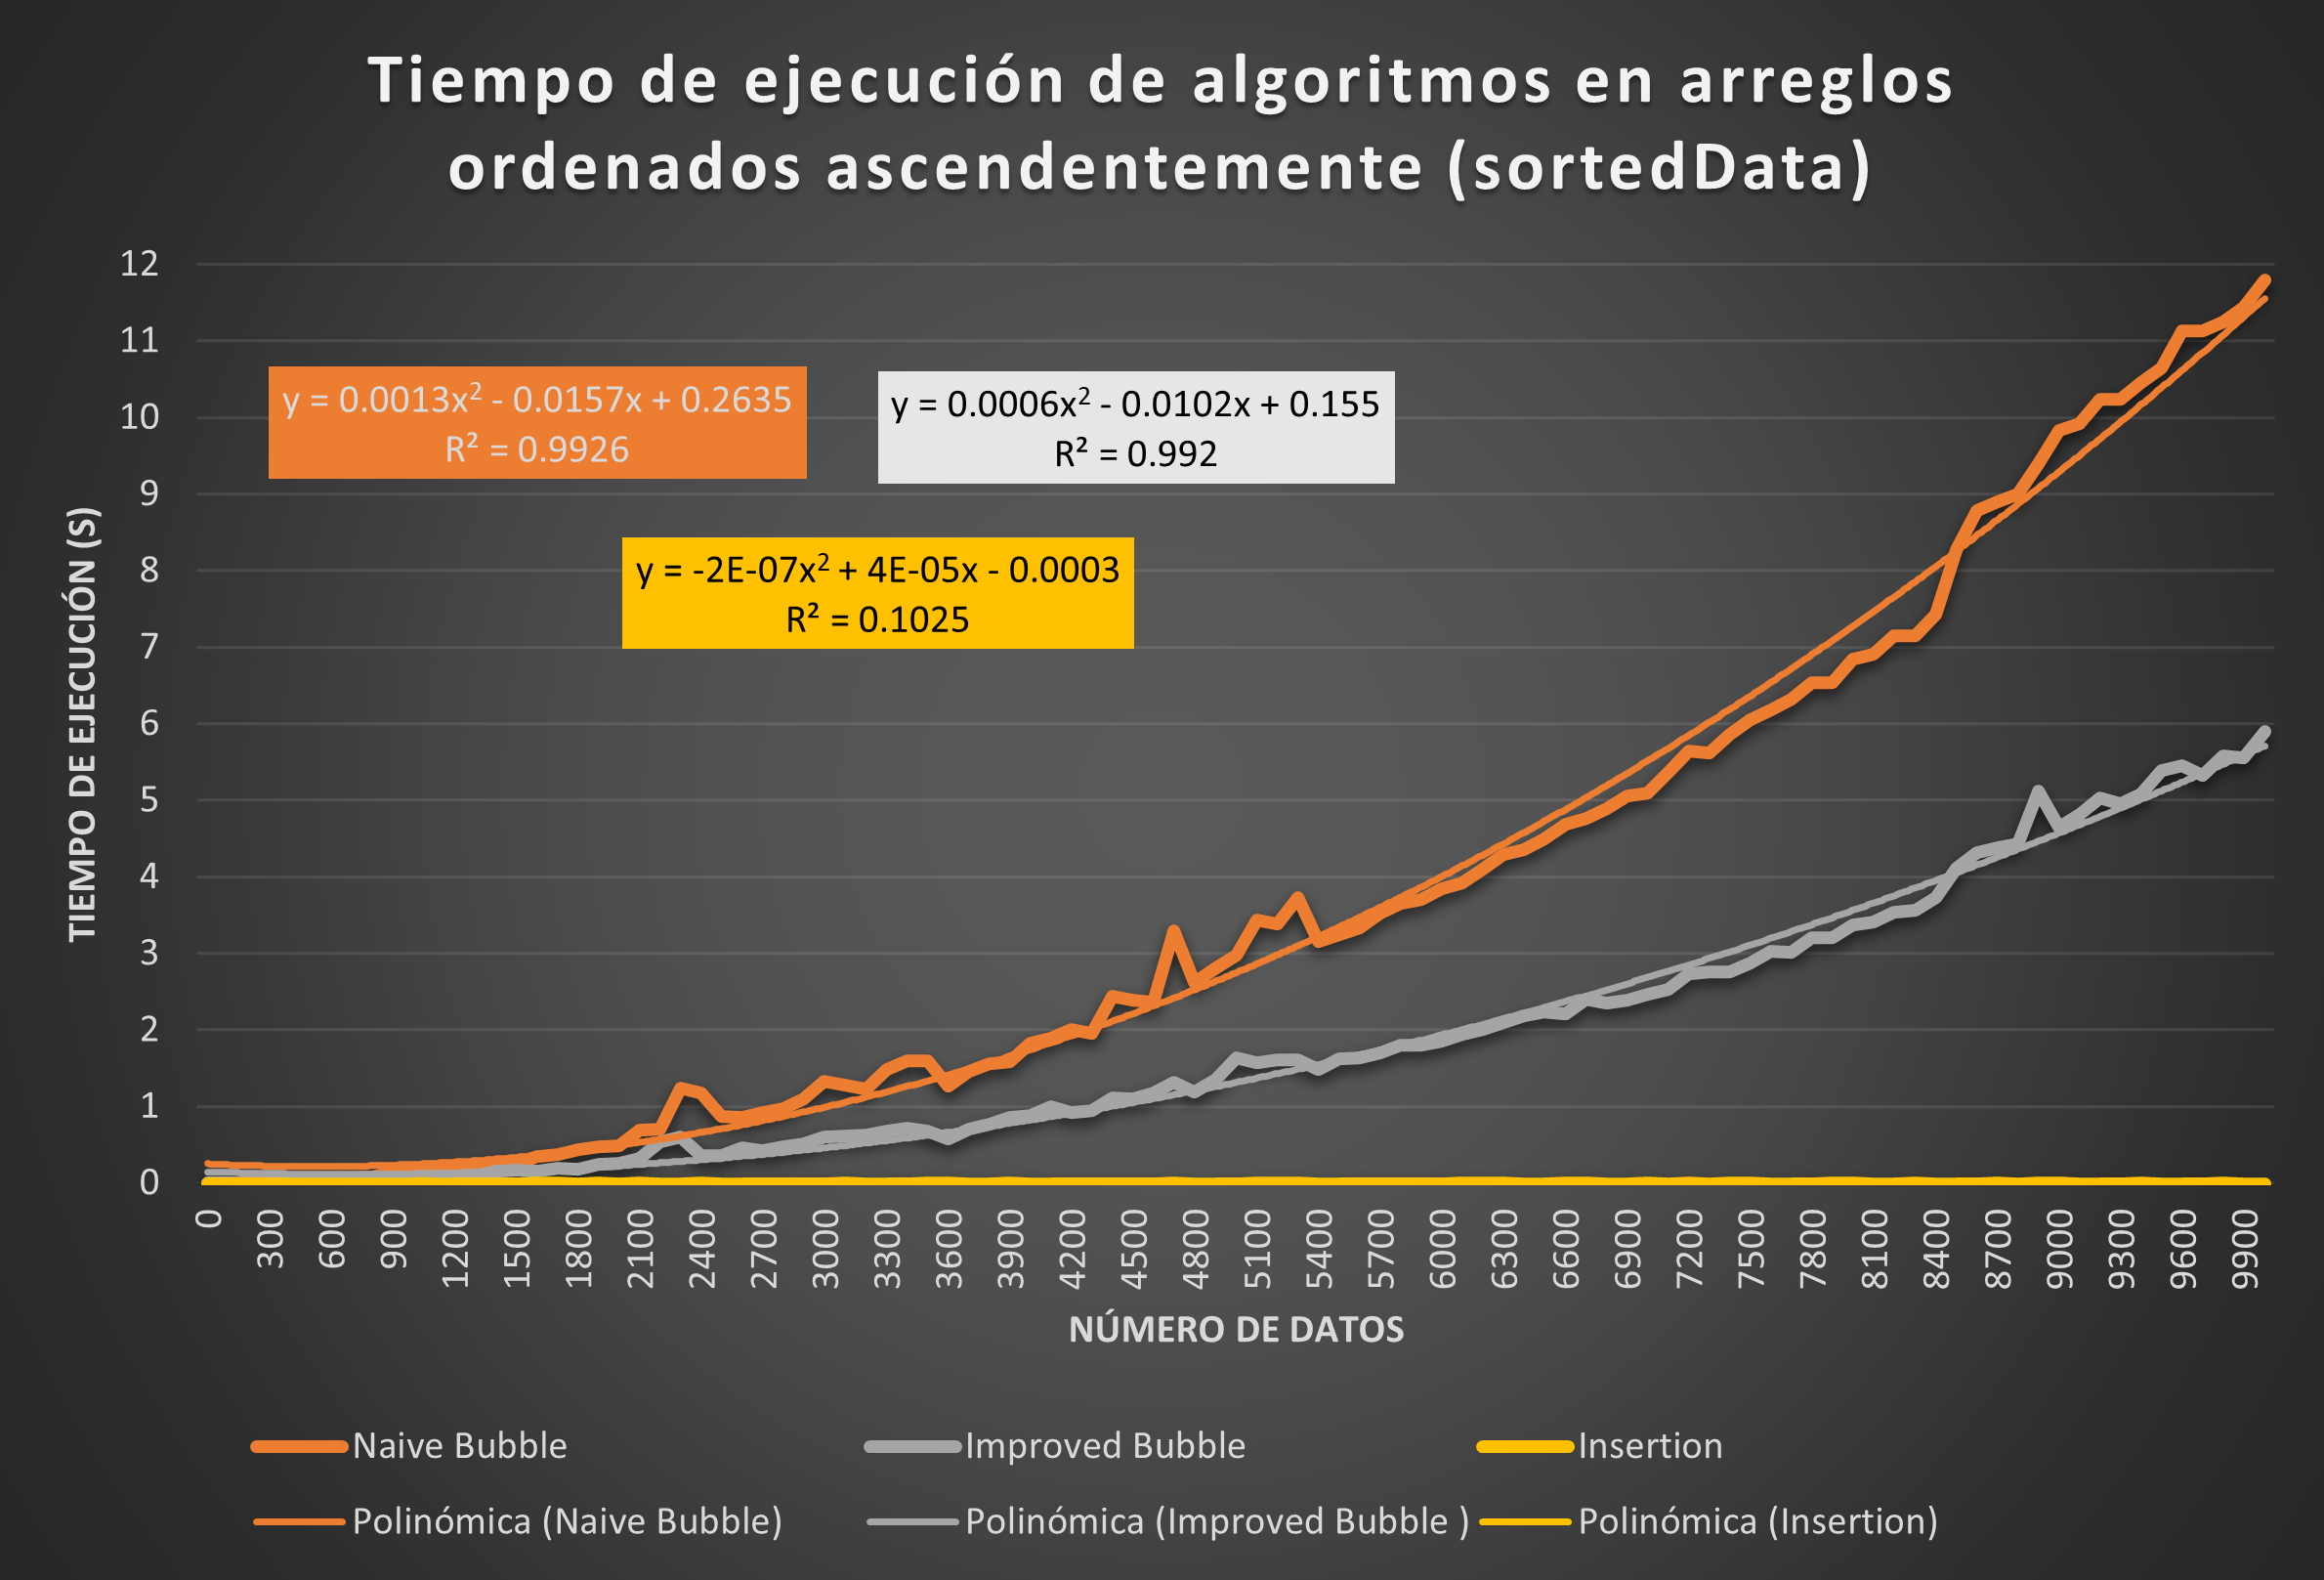
\includegraphics[scale=0.76]{sortedDataGraphic.png}
    \caption{Tiempo de ejecución de los algoritmos con datos ordenados ascendentemente}
   \label{experimentos:ordenadas:grafica}
\end{figure}

\subsubsection{Análisis del experimento}
\label{experimentos:ordenadas:analisis}
Una vez más, se evidencia la complejidad $\Theta(n^2)$ para $Bubble Sort$ en sus dos variantes; no obstante, mejora bastante el tiempo de ejecucicón, ya que pasa de un máximo de 14 segundos a 12 segundos aproximádamente.

Por otra parte, es clave notar el mejor caso para $Insertion Sort$. El hecho de que sea casi tangente al eje $x$ demuestra que su cota de complejidad inferior se cumple, siendo $\Omega(n)$.

Finalmente, haciendo un análisis de la regresión cuadrática aplicada a las curvas, se evidencia que el $Insertion Sort$ no deja de ser cuadrático, sin embargo, la constante que acompaña al $x^2$ es $-2^{-7}$ que tiende a 0, por tanto, ocasiona que se convierta en una función lineal, muy cercana al eje horizontal de la gráfica.


\subsection{Secuencias ordenadas invertidas} \label{experimentos:invertidas}

Acá se presentan los experimentos cuando los algoritmos se ejecutan con secuencias de entrada ordenadas de forma invertida de acuerdo al orden parcial $a<b$.

\subsubsection{Protocolo}
\begin{enumerate}
    \item Definir un rango $(b,e,s)\in\mathbb{N}^3$, donde: $b$ es un tamaño inicial, $e$ es un tamaño final y $s$ es un salto. Se generarán secuencias aleatorias de diferentes tamaños desde $b$ hasta $e$, adicionando cada vez $s$ elementos.
    \item Se usará el algoritmo \texttt{sort(S)} con el parámetro \texttt{reverse=True}, disponible en la librería básica de python, para ordenar dicha secuencia de manera descendente.
    \item Cada algoritmo se ejecutará 5 veces con cada secuencia ordenada y se guardará el tiempo promedio de ejecución.
    \item Se generan los gráficos necesarios para comparar los algoritmos.
\end{enumerate}

\subsubsection{Experimentación}
\begin{enumerate}
    \item Se utilizó el programa \texttt{$run\_reverse\_sorted\_experiment.py$} con los parámetros de entrada:
    \begin{itemize}
        \item \texttt{b=0} como tamaño inicial del arreglo
        \item \texttt{e=10000} como tamaño final del arreglo
        \item \texttt{s=100} como saltos entre iteraciones del algoritmo
    \end{itemize}
    \item Se creó un arreglo de tamaño \texttt{e} con números aleatorios entre -1000000 y 1000000.
    \item Utilizando la función \texttt{sort(S)} de la librería básica de Pyhton, junto con el parámetro \texttt{reverse=True}, se ordena descendentemente el arreglo y se empiezan a ejecutar los algoritmos. 
    \item El programa logró finalizar sin complicaciones, con un tiempo estimado de 2 horas y media.
    \item Se obtuvieron 100 datos con el tiempo promedio de cada uno de los algoritmos, logrando así crear la siguiente gráfica: (ver Figura 3)
\end{enumerate}

\begin{figure}[h]
    \centering
    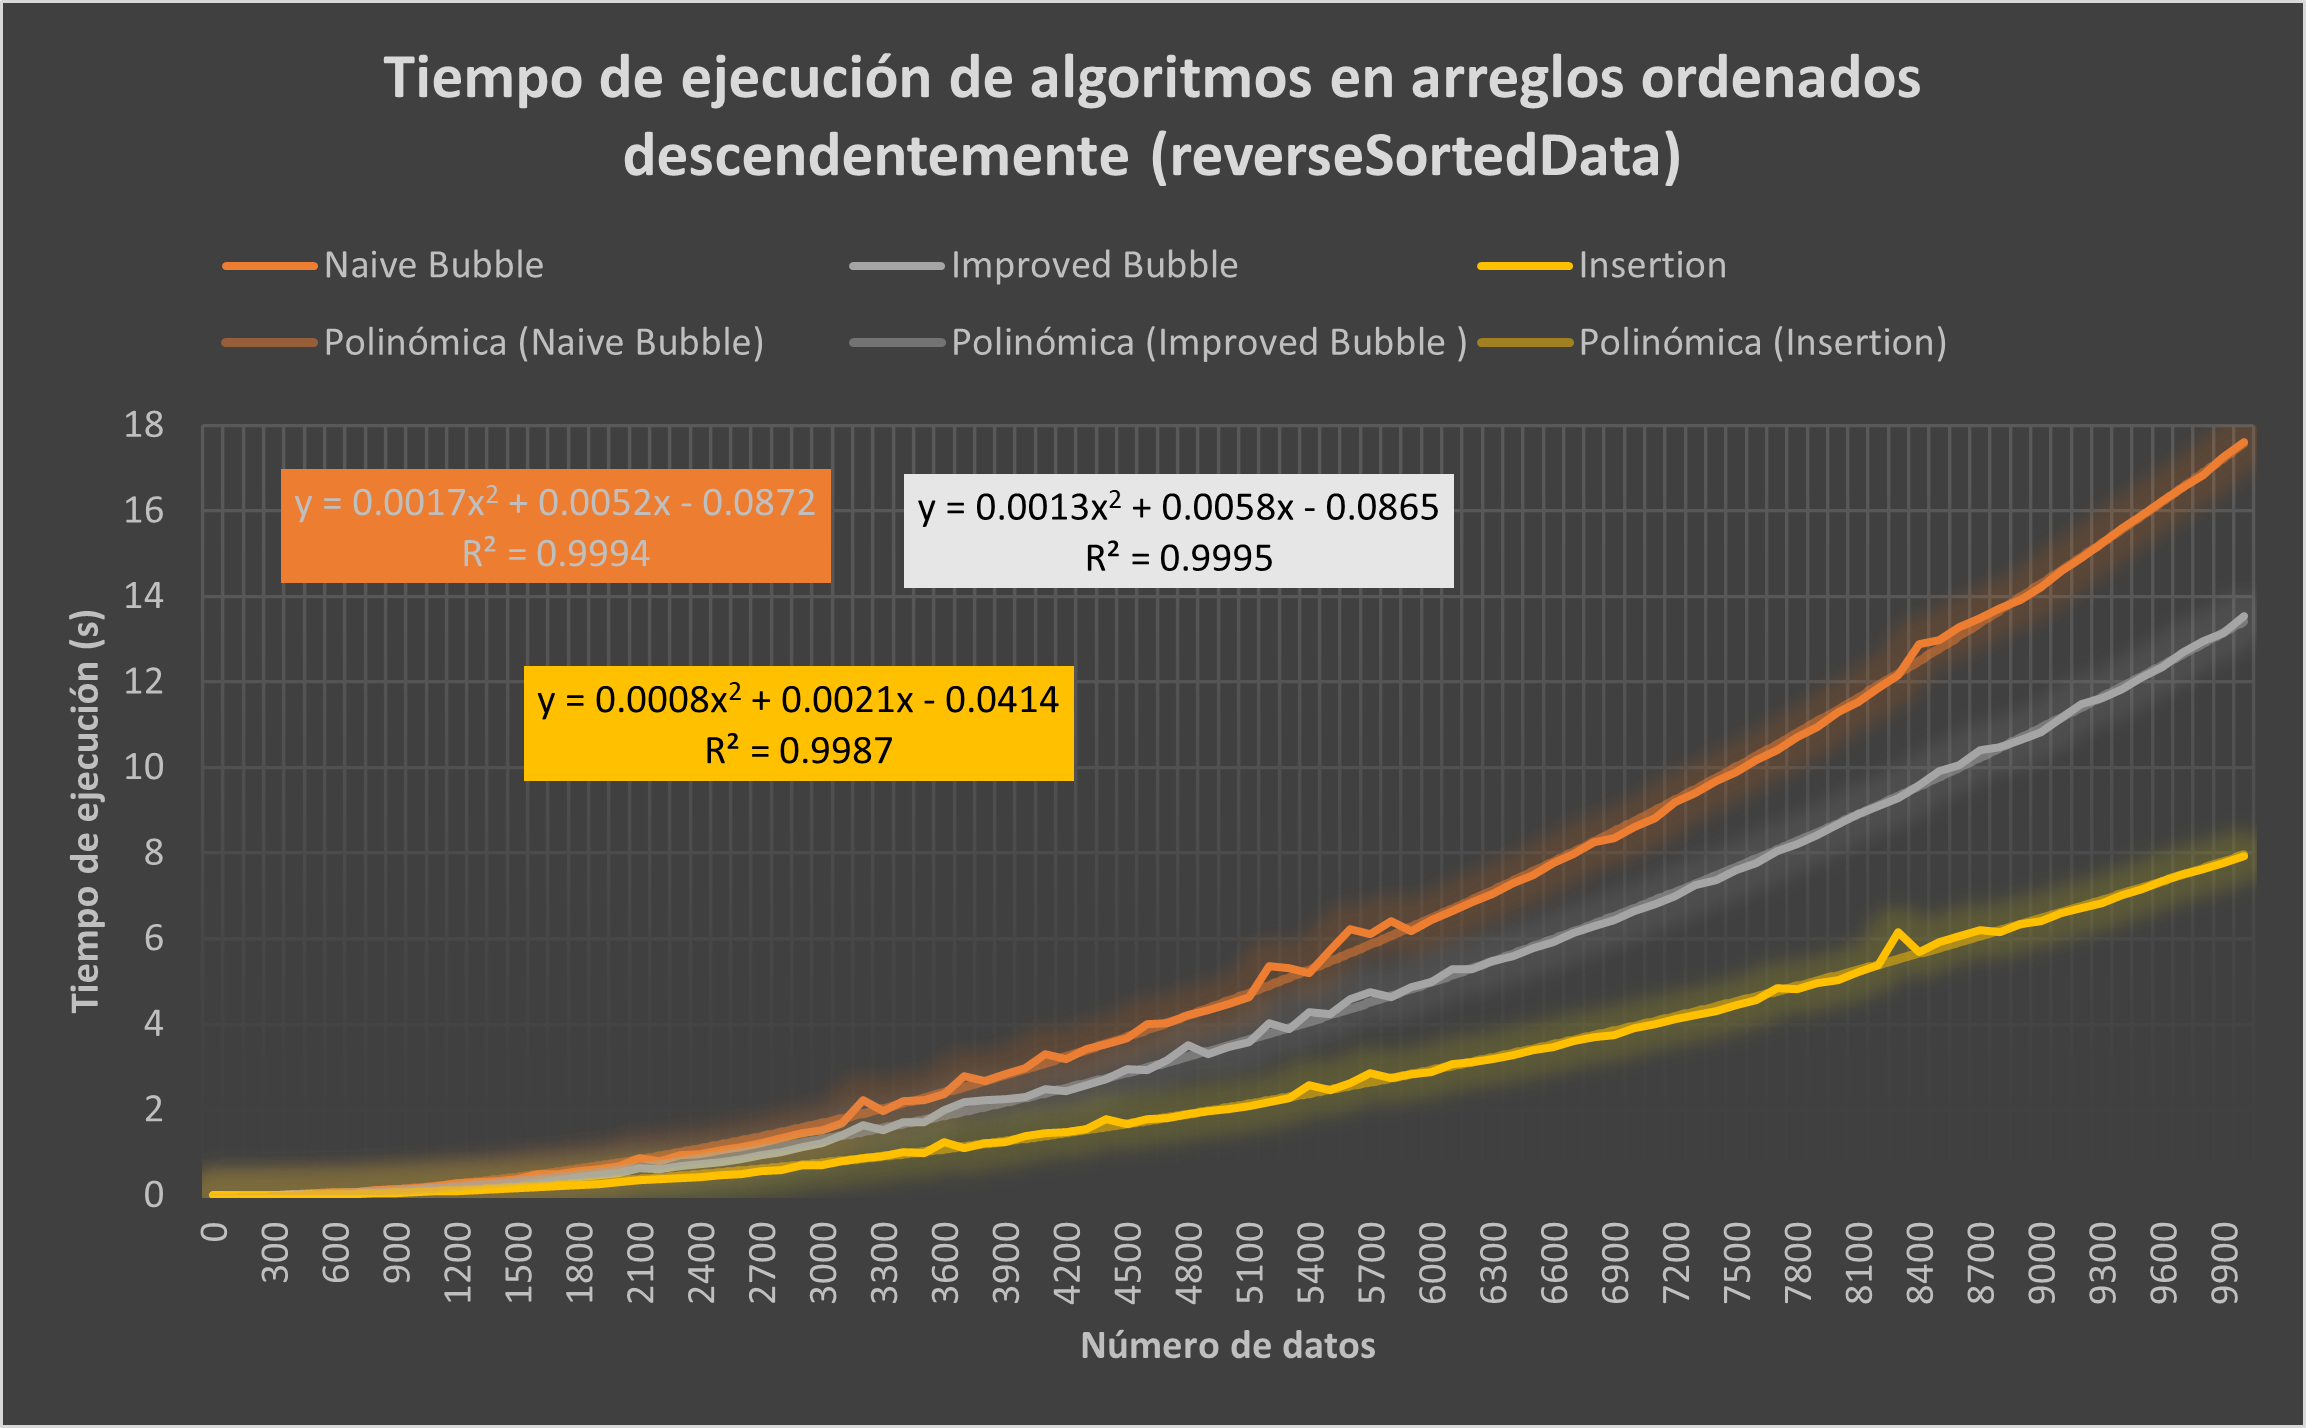
\includegraphics[scale=0.86]{reverseSortedDataGraphic.png}
    \caption{Tiempo de ejecución de los algoritmos con datos ordenados descendentemente}
   \label{experimentos:invertidas:grafica}
\end{figure}


\subsubsection{Análisis del experimento}
\label{experimentos:invertidas:analisis}
Para los 3 algoritmos, este fue el peor escenario. Fue el experimento donde las iteraciones tomaron más tiempo para lograr ordenar los arreglos debido a la invariante de los algoritmos, donde, en el caso de $Bubble Sort$ se busca ubicar los valores más grandes hacia el final del arreglo, y en $Insertion Sort$, se ajustan primero los  valores menores.

Es interesante cuestionarse qué tipo de algoritmo implementa \texttt{sort(S)} de Python, pues únicamente añadiendo el parámetro \texttt{reverse=True} se efectúa el ordenamiento descendente de manera casi instantánea.

Se consultaron algunas fuentes y se encontró que, ``desde la versión 2.3 de Python, éste usa el TimSort para ordenar los datos, un algoritmo que tiene una complejidad de $O(nlogn)$ siendo así uno basado en la estrategia de divide y vencerás, logrando su objetivo a velocidades prácticamente imperceptibles.'' \cite{Ed}

\section{Conclusiones}
Los experimentos fueron útiles para concluir:
\begin{enumerate}
    \item El tiempo de ejecución para el caso promedio (datos aleatorios) de estos algoritmos tiene una complejidad de $\Theta(n^2)$
    \item Insertion Sort tiene una cota de complejidad de $\Omega(n)$ si el arreglo está previamente ordenado de manera ascendente.
    \item Para todos los algoritmos, el peor caso es cuando el arreglo está previamente ordenado de manera descendente. Aquí, la cota de complejidad es $O(n^2)$.
    \item Los algoritmos estudiados en este taller funcionan de manera educativa para aprender sobre complejidad algorítmica, pero no deberían ser usados en un proyecto real. En ese caso, se podría optar por otros como el TimSort o el HeapSort.
\end{enumerate}

\begin{thebibliography}{X}
\bibitem{Ed} \textsc{Educative IO},
\textit{What is the Python list sort()?}, https://www.educative.io/answers/what-is-the-python-list-sort

\end{thebibliography}



\end{document}

%% eof - sorting.tex
